\documentclass[10pt,letterpaper]{article}
\usepackage[margin=0.75in]{geometry}
\usepackage{amsmath,amssymb,bm,array,booktabs,tabularx}
\usepackage[shortlabels]{enumitem}
\usepackage[dvipsnames]{xcolor}
\usepackage{fancyhdr}
\usepackage{tikz}
\setlength{\parindent}{0pt}
\setlength{\parskip}{0.34em}
\renewcommand{\arraystretch}{1.12}
\newcolumntype{Y}{>{\raggedright\arraybackslash}X}
\newcommand{\work}[1]{\vspace{#1}}
\definecolor{heat}{RGB}{165,67,38}
\definecolor{cool}{RGB}{22,111,119}
\pagestyle{fancy}
\fancyhf{}
\lhead{MA371: Project 1 Physics Inquiry}
\rhead{AY27-1}
\cfoot{\thepage}
\setlength{\headheight}{14pt}

\begin{document}
\begin{center}
{\Large\bfseries Two Modules, One Cool(ing) Decision}\\[3pt]
{\large Guided inquiry packet: Physics}
\end{center}
\textbf{Name:} \rule{2.4in}{0.4pt}\hfill
\textbf{Inquiry partners:} \rule{2.25in}{0.4pt}

\textbf{Decision brief.} A fictional portable communications unit has a heat-producing power module and a temperature-sensitive control module. Its program director can install \emph{one} modification: a powered ventilation kit or a passive thermal bridge between modules. Recommend one, recommend a limited test, or defer the choice. Your Army-style memo must connect the recommendation to predicted temperatures, physical reasoning, and the limits of the evidence. All equipment, parameters, and measurements are \textbf{synthetic teaching data}.

\textbf{Relevant MA371 connections.} Lesson 17: eigenvalues and eigenvectors. Lesson 18: diagonalization and eigenvector coordinates. Lesson 19 \& 20: linear systems of ordinary differential equations (ODEs) and modeling. This packet develops the heat-transfer model and scalar ODE ideas before applying those lessons. The physical concepts are introduced here, and the calculations use methods from MA371.

\textbf{Suggested class rhythm (50 minutes).} 8 minutes: one-module heat balance; 12: derive the two-module model; 12: interpret its two modes; 10: compare modifications; 8: challenge the prediction and frame a claim. Finish the memo and annex individually after class.

\section*{1. From heat flow to one differential equation}
When the unit is switched on, its temperature changes with time. Write $T(t)$ for the temperature at time $t$ and $T(0)$ for the measured starting temperature. The derivative $T'(t)$ is the slope of its temperature-versus-time curve: a positive value means warming at that instant. We use minutes for time, degrees Celsius for temperature, and kilojoules (kJ) for energy. One kJ/min is about $16.7$ watts.

The electronics produce heat at rate $P$. The module stores thermal energy as it warms; its \textbf{thermal capacity} $C$ tells us how many kilojoules correspond to a one-degree rise (approximately mass times specific heat). Heat conducts through the housing and is carried away by surrounding air through convection. We model this ambient loss by the \textbf{Newton cooling approximation} $h(T-T_a)$, where $T_a$ is ambient temperature. A greater temperature difference drives a greater heat flow, and stronger ventilation raises the effective coefficient $h$. If $T<T_a$, the signed heat flow reverses and the air warms the module. This \emph{lumped} model represents the module by one temperature and summarizes its housing and airflow with one coefficient.

\begin{center}
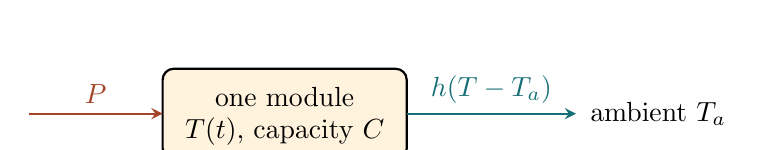
\begin{tikzpicture}[>=stealth,thick]
\draw[fill=Orange!13,rounded corners] (0,0) rectangle (3.1,1.15);
\node at (1.55,.79) {one module};
\node at (1.55,.35) {$T(t)$, capacity $C$};
\draw[->,heat] (-1.7,.58)--(0,.58) node[midway,above] {$P$};
\draw[->,cool] (3.1,.58)--(5.25,.58) node[midway,above] {$h(T-T_a)$};
\node[anchor=west] at (5.3,.58) {ambient $T_a$};
\end{tikzpicture}
\end{center}

\begin{tabularx}{\linewidth}{@{}p{0.69in}p{1.65in}Y@{}}
\toprule
Symbol & Units & Physical meaning\\
\midrule
$C$ & kJ/$^\circ$C & Thermal capacity: energy needed for a $1^\circ$C rise.\\
$P$ & kJ/min & Heat produced inside the module per minute.\\
$h$ & kJ/(min $^\circ$C) & Heat-loss coefficient; $h(T-T_a)$ is heat leaving per minute when $T>T_a$.\\
\bottomrule
\end{tabularx}

\textbf{Energy balance:} rate of stored thermal energy = rate produced $-$ rate lost. Since the stored energy changes by $C\,dT/dt$ kJ/min, a constant ambient temperature gives $d\theta/dt=dT/dt$ for $\theta=T-T_a$. Therefore
\[
\underbrace{C\frac{d\theta}{dt}}_{\text{kJ/min}}=P-h\theta.
\]\newpage
\textbf{Why an exponential solution appears.} At equilibrium, $\theta'=0$, so $\theta_*=P/h$. Subtract this constant equilibrium by setting $z(t)=\theta(t)-\theta_*$. The ODE becomes $z'=-(h/C)z$. Try the exponential ansatz $z(t)=Ke^{\lambda t}$. Substitution gives $\lambda K e^{\lambda t}=-(h/C)K e^{\lambda t}$, hence $\lambda=-h/C$. The initial temperature determines $K=T(0)-T_a-P/h$, so the predicted temperature is
\[
\boxed{T(t)=T_a+\frac{P}{h}+\left(T(0)-T_a-\frac{P}{h}\right)e^{-ht/C}.}
\]
\textbf{ Example.} Take $C=10$, $P=4$, $h=1$, $T_a=20^\circ$C, and $T(0)=20^\circ$C. The formula becomes $T(t)=24-4e^{-t/10}$ $({}^\circ\mathrm C)$. Check it: $T(0)=20$, while $C T'(t)=4e^{-t/10}=P-h(T(t)-T_a)$. Thus the function satisfies both the starting condition and the heat-balance ODE. Its time scale $C/h=10$ minutes is the time for the departure from equilibrium to shrink by a factor of $e^{-1}$.

\begin{enumerate}[a.,leftmargin=*]
\item At $t=0$, what is $dT/dt$ in $^\circ$C/min? What physical process makes that slope change later?\work{0.30in}
\item Evaluate $T(10)$ and explain why it is below $24^\circ$C even after one time scale.\work{0.30in}
\item If the module is initially \emph{above} its equilibrium temperature, which sign changes in the solution, and what happens to $T$?\work{0.27in}
\end{enumerate}

\newpage
\section*{2. Couple two modules through heat transfer}
Let $T_1$ be the power-module temperature and $T_2$ the control-module temperature. Each housing loses heat to ambient air by the cooling mechanism above. Each electronics module produces heat at rates $P_1$ and $P_2$ respectively. The thermal bridge conducts heat across the contact between housings: energy flows from the hotter module to the cooler one. We model that flow by $g(T_1-T_2)$. When $T_1>T_2$, this quantity is positive from module 1 to module 2. When their temperatures agree, the contact flow is zero. The conductance $g$ has the same units as $h$; a larger contact area or a more conductive bridge tends to increase it, while contact resistance reduces it.

\begin{center}
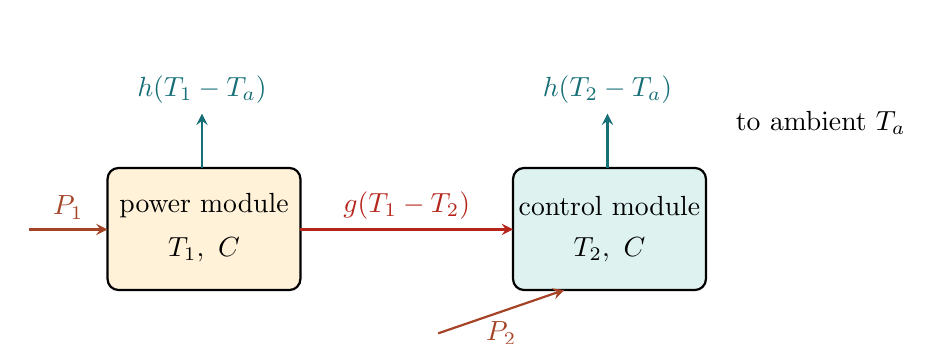
\begin{tikzpicture}[>=stealth,thick]
\draw[fill=Orange!15,rounded corners] (0,0) rectangle (2.45,1.55);
\draw[fill=TealBlue!15,rounded corners] (5.15,0) rectangle (7.6,1.55);
\node at (1.225,1.07) {power module}; \node at (1.225,.51) {$T_1,\ C$};
\node at (6.375,1.07) {control module}; \node at (6.375,.51) {$T_2,\ C$};
\draw[->,heat] (-1.0,.77)--(0,.77) node[midway,above] {$P_1$};
\draw[->,heat] (4.2,-.55)--(5.8,0) node[midway,below] {$P_2$};
\draw[->,BrickRed] (2.45,.77)--(5.15,.77) node[midway,above] {$g(T_1-T_2)$};
\draw[->,cool] (1.2,1.55)--(1.2,2.24) node[above] {$h(T_1-T_a)$};
\draw[->,cool] (6.35,1.55)--(6.35,2.24) node[above] {$h(T_2-T_a)$};
\node[anchor=west] at (7.85,2.12) {to ambient $T_a$};
\end{tikzpicture}
\end{center}

\textbf{Start with words.} For each module: stored-energy rate = internally produced heat $-$ heat lost to ambient $\mp$ heat exchanged with the other module. The bridge transfers equal amounts out of one module and into the other. We assume equal capacities $C$ and equal ambient-loss coefficients $h$ for this initial model; that symmetry will make the two temperature patterns easy to interpret.

For $\theta_i=T_i-T_a$, the first balance is
\[
C\theta_1'=P_1-h\theta_1-g(\theta_1-\theta_2).
\]
\begin{enumerate}[a.,leftmargin=*]
\item Write the balance for module 2. Why must the contact term have the opposite sign?\work{0.40in}
\item Add the two balances. Which terms cancel, and what does that say about a passive bridge's ability to remove heat from the \emph{whole} unit?\work{0.46in}
\item Suppose $T_1=T_2>T_a$. Which heat flow becomes zero? Which flows continue?\work{0.32in}
\end{enumerate}

\textbf{Matrix checkpoint.} After deriving both balances, verify that your result matches
\[
\underbrace{\frac{d\vec\theta}{dt}}_{2\times1}=
\underbrace{\frac{1}{C}
\begin{bmatrix}-(h+g)&g\\g&-(h+g)\end{bmatrix}}_{A\,\text{in min}^{-1}}
\underbrace{\vec\theta}_{2\times1}
+\underbrace{\frac1C\begin{bmatrix}P_1\\P_2\end{bmatrix}}_{\vec b\,\text{in }^\circ\mathrm C/\text{min}},
\qquad \vec\theta=\begin{bmatrix}\theta_1\\\theta_2\end{bmatrix}.
\]
The matrix tells us how current temperature differences affect \emph{rates}; $\vec b$ represents ongoing heat production. Determine each module's warming or cooling from its complete energy balance.

\textbf{Baseline case.} Use $C=10$ kJ/$^\circ$C, $h=1$ kJ/(min $^\circ$C), $g=0.5$ kJ/(min $^\circ$C), $P_1=20$ kJ/min, $P_2=4$ kJ/min, $T_a=20^\circ$C, and $T_1(0)=T_2(0)=20^\circ$C.
\begin{enumerate}[d.,leftmargin=*]
\item Fill the numerical $A$ and $\vec b$. Check the units of one term in each equation.\work{0.43in}
\item At the instant power turns on, find $T_1'(0)$ and $T_2'(0)$. Is there contact heat flow at that instant? What happens immediately afterward?\work{0.39in}
\end{enumerate}

\newpage
\section*{3. See eigenvectors as physical temperature patterns}
Lesson 19 used the homogeneous system $\vec x'=A\vec x$. Here constant heat production adds the term $\vec b$. Find an equilibrium $\vec\theta_*$ satisfying $A\vec\theta_*+\vec b=\vec0$, then track displacement from it: $\vec z=\vec\theta-\vec\theta_*$ satisfies $\vec z'=A\vec z$. Its eigenmodes describe how departures from equilibrium fade. For equipment starting at ambient, that decay accompanies a rise in absolute temperature.

The physical patterns become clear in the sum and difference
\[
s=\theta_1+\theta_2 \quad\text{(overall temperature elevation)},\qquad
d=\theta_1-\theta_2 \quad\text{(temperature contrast)}.
\]
From the two balances, derive and then check
\[
s'=-\frac{h}{C}s+\frac{P_1+P_2}{C},\qquad
d'=-\frac{h+2g}{C}d+\frac{P_1-P_2}{C}.
\]
The bridge terms cancel in the equation for $s$ and reinforce each other in the equation for $d$. Contact redistributes heat within the unit; ambient cooling removes heat from it.

\begin{enumerate}[a.,leftmargin=*]
\item Explain why a larger $g$ makes a temperature contrast disappear faster but leaves the \emph{average-mode decay rate} unchanged in this symmetric model.\work{0.43in}
\item Check directly that $\vec v_+=(1,1)^T$ and $\vec v_-=(1,-1)^T$ are eigenvectors of $A$. Fill in their eigenvalues and units:
\[
A\vec v_+=\lambda_+\vec v_+,\quad\lambda_+=\rule{1.2in}{0.4pt};\qquad
A\vec v_-=\lambda_-\vec v_-,\quad\lambda_-=\rule{1.2in}{0.4pt}.
\]
\item For the baseline, compare the decay factors $e^{\lambda_+t}$ and $e^{\lambda_-t}$. Which pattern fades faster? Explain how the negative eigenvalues describe the approach to equilibrium while the powered modules warm from $20^\circ$C.\work{0.55in}
\end{enumerate}
\newpage
The curves below trace the \emph{fraction of an initial departure from equilibrium remaining}. Match the solid and dashed curves to the two baseline modes; explain your choice using the eigenvalues.
\begin{center}
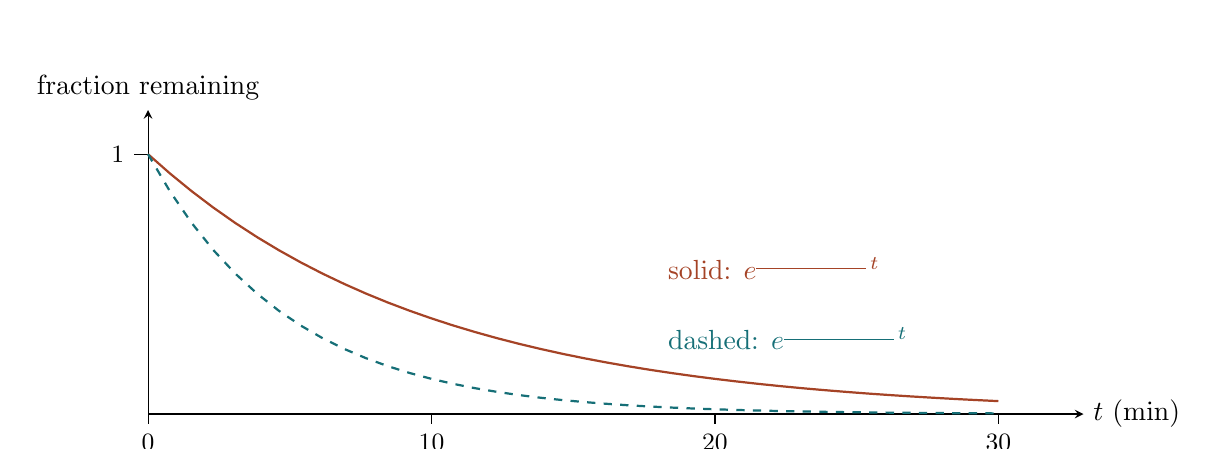
\begin{tikzpicture}[x=.36cm,y=3.3cm,>=stealth]
\draw[->] (0,0)--(33,0) node[right] {$t$ (min)};
\draw[->] (0,0)--(0,1.17) node[above] {fraction remaining};
\foreach \x in {0,10,20,30} {\draw (\x,0)--(\x,-.04) node[below] {\small\x};}
\draw (0,1)--(-.5,1) node[left] {\small 1};
\draw[heat,thick,domain=0:30,samples=40] plot (\x,{exp(-\x/10)});
\draw[cool,thick,dashed,domain=0:30,samples=40] plot (\x,{exp(-\x/5)});
\node[heat,anchor=west] at (18,.56) {solid: $e^{\rule{.55in}{.4pt}\,t}$};
\node[cool,anchor=west] at (18,.29) {dashed: $e^{\rule{.55in}{.4pt}\,t}$};
\end{tikzpicture}
\end{center}

For a scalar ODE $y'=-ay+f$ with $a>0$, the equilibrium is $y_*=f/a$ and
\[
y(t)=y_*+\bigl(y(0)-y_*\bigr)e^{-at}.
\]
Our modules start at ambient, so $s(0)=d(0)=0$. Applying the scalar formula gives the \textbf{calculation bridge}
\[
s(t)=\frac{P_1+P_2}{h}\bigl(1-e^{-ht/C}\bigr),\qquad
d(t)=\frac{P_1-P_2}{h+2g}\bigl(1-e^{-(h+2g)t/C}\bigr),
\qquad
\theta_1=\frac{s+d}{2},\quad\theta_2=\frac{s-d}{2}.
\]
The fractions preceding the exponentials are the steady values $s_*$ and $d_*$. They also provide a physical check of $\vec\theta_*=-A^{-1}\vec b$.

\begin{enumerate}[d.,leftmargin=*]
\item Use $s_*$ and $d_*$ to find the baseline equilibrium temperatures $T_{1,*}$ and $T_{2,*}$. State why $T_{1,*}>T_{2,*}$.\work{0.47in}
\item Write $\vec\theta(t)=\vec\theta_*+c_+e^{\lambda_+t}\vec v_++c_-e^{\lambda_-t}\vec v_-$. Determine $c_+$ and $c_-$ from $\vec\theta(0)=\vec0$; verify the same answer using $s(t),d(t)$.\work{0.55in}
\end{enumerate}

\newpage
\section*{4. Compare modifications at the relevant time}
The director expects a \textbf{30-minute operation} but wants to understand what a longer run would change. At the nominal $20^\circ$C ambient temperature, the limits are $T_1\le34.5^\circ$C for the power module and $T_2\le29.0^\circ$C for the control module. Exactly one modification may be installed; $C,P_1,P_2$ remain as stated.

\begin{center}
\begin{tabularx}{\linewidth}{@{}p{0.75in}p{1.68in}p{1.45in}Y@{}}
\toprule
Case & Changed coefficient & Physical action & Operational consideration\\
\midrule
Baseline & $h=1,\ g=0.5$ & No modification & No added load.\\
Ventilation & $h=1.35,\ g=0.5$ & Removes heat faster to ambient. & Draws $25$ W from the power supply; filter upkeep.\\
Bridge & $h=1,\ g=1.0$ & Moves heat between modules faster. & Passive; added mass and uncertain contact quality.\\
\bottomrule
\end{tabularx}
\end{center}
In the model, the fan's electrical draw is an operational cost. We assume its motor heat is rejected outside the two modules, so $P_1$ and $P_2$ remain fixed.

\textbf{Worked setup.} In the baseline at $t=30$ min, $ht/C=3$ and $(h+2g)t/C=6$, so
\[
s(30)=24(1-e^{-3}),\qquad d(30)=8(1-e^{-6}).
\]
Evaluate these before converting back to temperatures. Keep unrounded values through the calculation; round only the reported temperatures.

\begin{enumerate}[a.,leftmargin=*]
\item Compute baseline $T_1(30)$ and $T_2(30)$ by hand. Which limit matters?\work{0.57in}
\item Before calculating, predict what raising $h$ does to the \emph{overall} temperature and what raising $g$ does to the \emph{difference} $T_1-T_2$. Could the bridge make the control module warmer?\work{0.52in}
\end{enumerate}

Use the same formulas for the two modifications. Record numerical evidence and units in the table; a later calculator can help you visualize the curves and check your arithmetic.
\begin{center}
\begin{tabular}{@{}lcccc@{}}
\toprule
Case & $T_1(30)$ ($^\circ$C) & $T_2(30)$ ($^\circ$C) & $T_{1,*}$ ($^\circ$C) & $T_{2,*}$ ($^\circ$C)\\
\midrule
Baseline & \rule{.70in}{.4pt} & \rule{.70in}{.4pt} & \rule{.70in}{.4pt} & \rule{.70in}{.4pt}\\[8pt]
Ventilation & \rule{.70in}{.4pt} & \rule{.70in}{.4pt} & \rule{.70in}{.4pt} & \rule{.70in}{.4pt}\\[8pt]
Bridge & \rule{.70in}{.4pt} & \rule{.70in}{.4pt} & \rule{.70in}{.4pt} & \rule{.70in}{.4pt}\\
\bottomrule
\end{tabular}
\end{center}

\begin{enumerate}[c.,leftmargin=*]
\item Mark each case as meeting or missing \emph{both} 30-minute limits. Are the results at $t=30$ and at equilibrium necessarily the same decision? Explain what the latter means physically.\work{0.47in}
\item A negative eigenvalue signals a decaying \emph{mode}. What additional information determines whether the director's temperature limits are met?\work{0.41in}
\end{enumerate}

\newpage
\section*{5. Draw the prediction, then challenge the model}
The points below are \textbf{synthetic held-out bench observations} for the \emph{baseline unit}. These readings were reserved as a check on the previously selected coefficients $C,h,g,P_1,P_2$. All three time readings come from the same device.
\begin{center}
\begin{tabular}{@{}lrrr@{}}
\toprule
Time after turn-on (min) & 10 & 20 & 30\\
\midrule
Measured power-module $T_1$ ($^\circ$C) & 31.2 & 34.6 & 35.8\\
Measured control-module $T_2$ ($^\circ$C) & 24.1 & 26.5 & 27.5\\
\bottomrule
\end{tabular}
\end{center}

\begin{center}
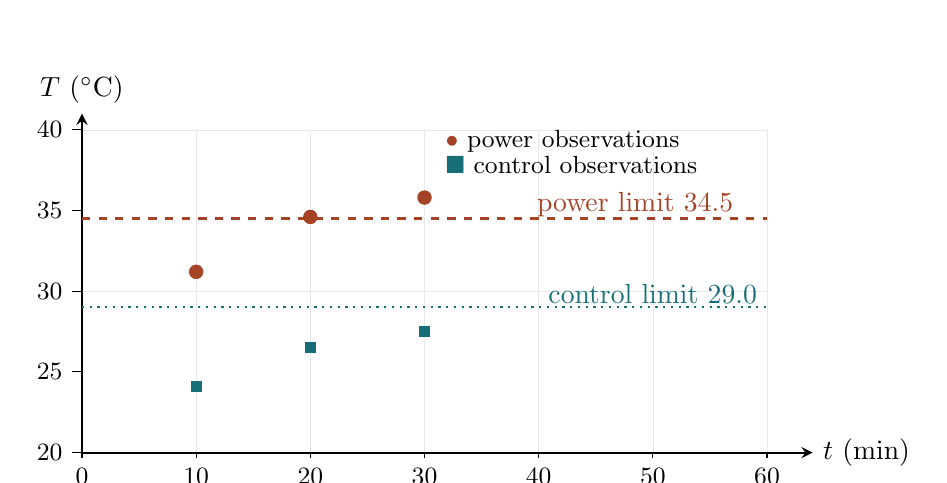
\begin{tikzpicture}[x=.145cm,y=.205cm,>=stealth]
\draw[step=10,gray!18,very thin] (0,20) grid (60,40);
\draw[->,thick] (0,20)--(64,20) node[right] {$t$ (min)};
\draw[->,thick] (0,20)--(0,41) node[above] {$T$ ($^\circ$C)};
\foreach \x in {0,10,20,30,40,50,60} {\draw (\x,20)--(\x,19.65) node[below] {\small\x};}
\foreach \y in {20,25,30,35,40} {\draw (0,\y)--(-.85,\y) node[left] {\small\y};}
\draw[heat,dashed,thick] (0,34.5)--(60,34.5);
\draw[cool,dotted,thick] (0,29)--(60,29);
\node[heat,anchor=west] at (39,35.35) {power limit $34.5$};
\node[cool,anchor=west] at (40,29.85) {control limit $29.0$};
\foreach \x/\y in {10/31.2,20/34.6,30/35.8} {\node[draw=heat,fill=heat,circle,inner sep=1.7pt] at (\x,\y) {};}
\foreach \x/\y in {10/24.1,20/26.5,30/27.5} {\node[draw=cool,fill=cool,rectangle,inner sep=1.8pt] at (\x,\y) {};}
\node[anchor=west] at (31,39.3) {\small \textcolor{heat}{$\bullet$} power observations};
\node[anchor=west] at (31,37.8) {\small \textcolor{cool}{$\blacksquare$} control observations};
\end{tikzpicture}
\end{center}

\begin{enumerate}[a.,leftmargin=*]
\item On the axes, sketch your \emph{baseline model} curves through $t=30$, using your $t=10,20,30$ predictions. Label the modeled curves separately from the measured points. Do they rise toward equilibrium as expected?\work{0.16in}
\item Compute the observed-minus-predicted residual for each module at $t=30$. What does its sign mean? What does an ODE-solution residual test, and what evidence evaluates physical prediction accuracy?\work{0.49in}
\item Compare the size of the baseline model's 30-minute discrepancy with the bridge's \emph{modeled} margin below each limit. Can one baseline bench run certify the bridge's field performance?\work{0.48in}
\end{enumerate}

\textbf{Hotter-day sensitivity.} Suppose the equipment starts equilibrated to a constant $22^\circ$C ambient temperature instead of $20^\circ$C. Assume the coefficients and heat inputs remain unchanged. Because $\vec\theta(0)=\vec0$ in both cases, each \emph{absolute} modeled temperature curve shifts upward by $2^\circ$C.
\begin{enumerate}[d.,leftmargin=*]
\item Use the $2^\circ$C shift to reassess both modifications at 30 minutes. Which appears more robust to this change? Which physical effects could alter $h$, $g$, or heat production on a hotter day?\work{0.45in}
\item Propose one additional bench or field measurement that would most reduce uncertainty before adopting a modification. State the outcome, comparison, and relevant operating condition.\work{0.42in}
\end{enumerate}

\newpage
\section*{6. Turn exploration into a decision memo}
\textbf{Before leaving class, record your own claim.} A conditional recommendation is appropriate if a predicted temperature lies close to a limit or depends on an untested heat-transfer assumption.
\begin{center}
\begin{tabularx}{\linewidth}{@{}p{1.82in}Y@{}}
\toprule
Claim and decision criterion & \rule{0pt}{0.43in}\\
\\
\\
\midrule
ODE and temperature evidence & \rule{0pt}{0.55in}\\
\\
\\
\midrule
Physical limitation or contrary evidence & \rule{0pt}{0.55in}\\
\\
\\
\midrule
Measurement needed next & \rule{0pt}{0.45in}\\
\\
\\
\bottomrule
\end{tabularx}
\end{center}

\textbf{Final product (typed).} Write an Army-style memo of at most two pages to the program director. Recommend ventilation, the bridge, a conditional pilot, or deferral. Clearly state the 30-minute temperature criterion, the relevant numerical comparison, the ventilation power tradeoff, and a limitation in language a nontechnical leader can use. Label \emph{modeled predictions} and measured outcomes clearly. A due date and submission method will be provided by the instructor.

Attach a \textbf{separate technical annex of at most three pages} that makes the claim auditable: the heat-balance derivation and units; $A,\vec b$ and initial state; equilibrium and one eigenpair check; a labeled temperature-versus-time figure or table for all cases; held-out residuals and hotter-day sensitivity. Use the annex to explain the physics and calculation. Select the algebraic steps that substantiate your claim.

\textbf{AI as a classroom coach (optional).} During the designated class inquiry, an approved AI tool may explain a derivative, question a sign convention, or critique an inference. Verify its claims against the balance equations, units, and supplied measurements. Record the tool, purpose, assistance, and how you checked it. Use only this synthetic case with AI tools. The final memo and annex are \emph{independently authored}: do your own outlining, drafting, rewriting, editing, and figure captions. Typing and the supplied numerical calculator are allowed.

\textbf{One final physical check.} In one or two sentences, explain why increasing thermal contact $g$ can help the hot module yet harm the cooler module, whereas increasing ventilation $h$ removes energy from the whole two-module system.\work{0.58in}

\end{document}

